The Langevin equation is a stochastic differential equation (SDE) originally developed to model the movement of a Brownian particle 	\cite{Langevin1908}. The form of interest here is the \emph{overdamped} Langevin equation, in which the particle experiences no average acceleration. The equation is thus
	\begin{equation} \dif X_t = -\nabla U(X_t)\dif t +\sqrt{2}\dif W_t. \label{eq:ODLang}\end{equation}
Here, \(W_t\) is a \(d\)-dimensional Wiener process (Brownian motion) and \(U:\R^d \to \R\) is the potential function. The equation can be thought of as modelling a particle in a potential well with shape \(U\). As each particle moves randomly, it is natural to ask what is the average position of many particles in such a well? It can be shown that in fact the position of a particle moving according to the above dynamics is exactly \(\pi\) +++Reference to earlier section/first mention of distribution+++. For a diffusion process this is called the \emph{stationary distribution}\footnote{Another common term is \emph{invariant measure} +++} To show that \(\pi\) is indeed the stationary distribution the following lemma

\begin{lemma}
	For a one-dimensional It\^o diffusion,
	\[\dif X_t = \mu(X_t)\dif t + \sigma^2(X_t)dW_t,\]
	the Fokker-Planck operator, \(\L^*\), is
	\[\L^*:= -\partial_x(\mu(x)\cdot)+\frac{1}{2}\partial^2_x(\sigma^2(x)\cdot).\]
	A measure \(\pi\) is invariant for the diffusion if and only if
	\[\L^*\pi = 0\]
\end{lemma}
The proof of this is omitted however it can be seen by forming the Fokker-Planck equation for the probability density of the diffusion. The proof that \(\pi\) is the stationary measure of Equation \eqref{eq:ODLang} is given only in the one dimensional case, however it is extendable to higher dimensions. For the Langevin equation, the Fokker-Planck operator is

\[\L^* = \partial_x(U'(x)\cdot)+\partial_{xx}\cdot . \]
So it remains to calculate \(\L^*\pi\). 
\begin{align*}
\L^*\pi &= \pd{}{x}\bigg\lbrack U'(x)\pi(x) + \pd{}{x}\pi(x)\bigg\rbrack\\
		&= \pd{}{x}\bigg\lbrack U'(x)\mathcal{Z}\e^{-U(x)}+ \left(-U'(x)\mathcal{Z}\e^{-U(x)}\right)\bigg\rbrack\\
		&= \pd{}{x}\lbrack 0 \rbrack\\
		&= 0
\end{align*}
Hence \(\pi\) is indeed the invariant measure of \eqref{eq:ODLang}. \qed 
\\
\\
Although this shows that the Langevin equation has an invariant measure, the question of convergence to this measure remains unanswered. Roberts and Tweedie give the following restriction \cite{RT96}.
\begin{theorem}[Theorem 2.1, \cite{RT96}]
	Let \(P^t_X(x,A) = \P(X_t\in A | X_0 =x_0)\) and suppose that \(\grad U(x)\) is continuously differentiable and that, for some \(N,a,b < \infty\),
	\[\grad U(x)\cdot x \leq a|x|^2 + b, \qquad |x|>N. \]
	Then the measure \(\pi\) is invariant for the Langevin diffusion \(X\). Moreover, for all \(x \in \R^d \) and Borel sets \(A\),
	\[\|P^t_X(x,\cdot) - \pi \| = \frac{1}{2}\sup_A \big|P^t_X(x,A)-\pi(A)\big| \to 0\]

\end{theorem}
+++Should this norm be an integral? Add exponentially fast convergence/spectral gap inequality? Figure of \(U=x^2/2\)? 2d?  +++\\

\begin{figure}[h]
	\centering
		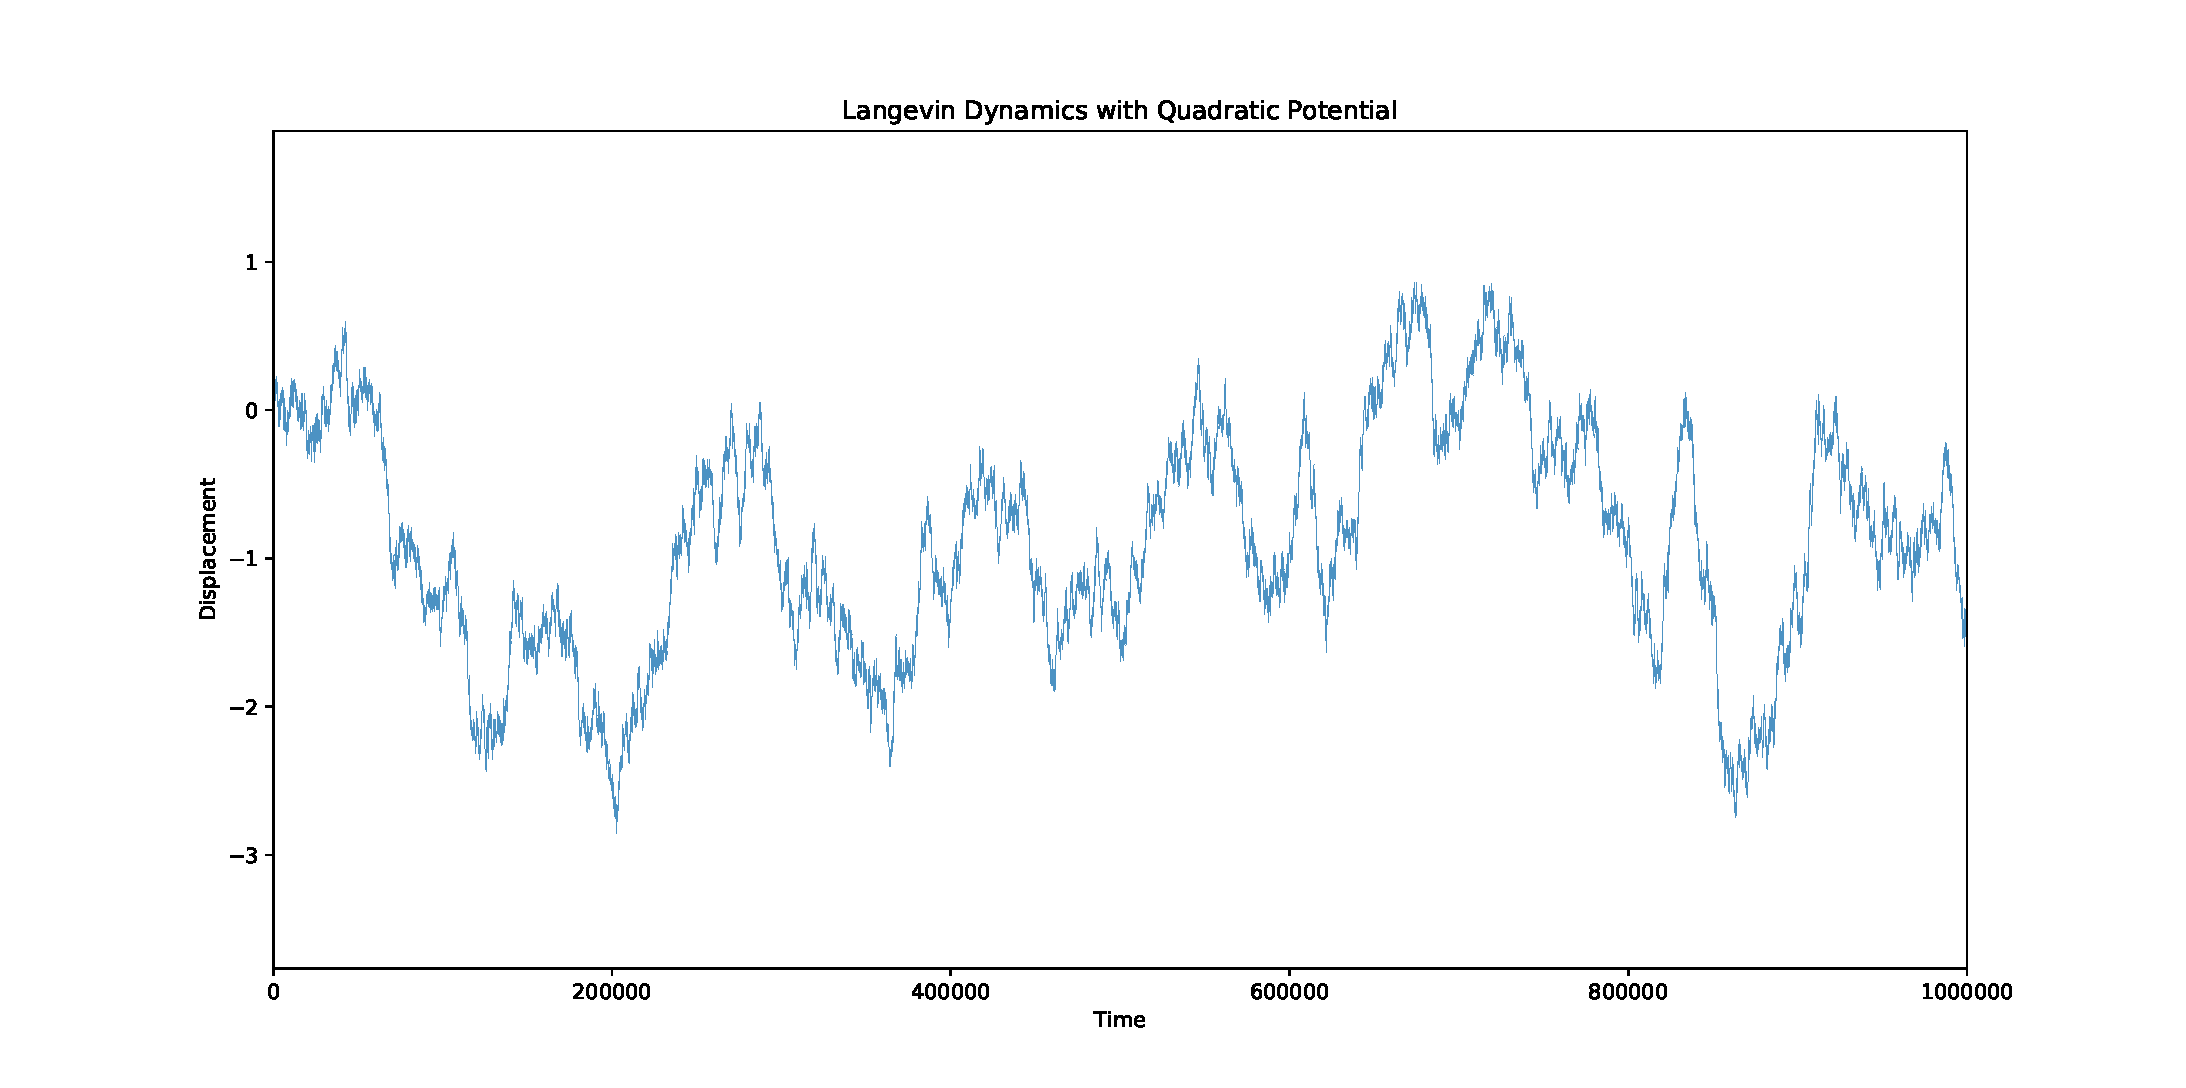
\includegraphics[width=\linewidth]{quadraticLD.pdf}
	\caption{Simulating Langevin dynamics in one dimension with a quadratic potential \(U(x)=x^2/2\)}
	\label{fig:quadLD}
\end{figure} 

The problem of sampling from the high dimensional distribution has been reduced to being able to accurately simulate Langevin dynamics. However, this is not as simple as it sounds. To simulate the continuous process  \eqref{eq:ODLang}, it must first be discretised. However, doing so may not preserve the convergence to the invariant measure. The discretised process may not have the same stationary measure or the masure may not even exist. This means that the method used to discretise must be chosen carefully to ensure good convergence properties. The most natural way to discretise an SDE is to use the stochastic analogue of the Euler method used on ordinary differential equations, known as the Euler-Maruyama (EM) method. Doing so leads to the Unadjusted Langevin Algorithm (\texttt{ULA}).

\subsection{The Unadjusted Langevin Algorithm}
Applying the Euler-Maruyama method to Equation \eqref{eq:ODLang} gives the following iterative scheme.

\[X_{n+1} = X_n -h \nabla U(X_n) +\sqrt{2h} Z_{n+1},\qquad X_0= x_0 \]
Here the \(Z_n \) are i.i.d. standard normal random variables and \(h\) is the step size. This is equivalent to \(X_{n+1} \sim N(X_n - h\grad U(X_n), 2h I_d )\).\footnote{\(I_d\) denotes the \(d \times d\) identity matrix.} A simple example shows that this discretisation does not converge to \(\pi\). Let \(\pi\) be a standard Gaussian distribution, that is \(U(x) = |x|^2/2 \) and choose \(h = 1\). Then the update is given by 

\begin{align*}
	X_{n+1} &\sim N(X_n - \grad U(X_n), 2)\\
	& \sim  N(X_n - X_n, 2)\\
	& \sim N(0,2) \nsim \pi .
\end{align*}
So the chain converges immediately, but to the wrong distribution. Let \(\pi^{\text{ULA}}_{h} \) denote the stationary distribution of \texttt{ULA} with a stepsize \(h\). This is not the only issue that can occur. As well as not converging to the correct distribution, the discretised chain may not be  ergodic, even when the continuous diffusion is exponentially ergodic \cite{RT96}. In particular, the algorithm misbehaves when the gradient of the potential is superlinear. That is,
\[\liminf_{\|x\|\to \infty} \frac{\|\grad U(x)\|}{\|x\|} = +\infty. \]
To mitigate these issues there are two main approaches: taming the gradient and Metropolisation. A further third method involves using a different discretisation scheme.  Our main focus will be the former, although all three approaches will be discussed. 

\section{MALA}
Before describing the Metropolis-adjusted Langevin algorithm \texttt{MALA}, it is pertinent at this point to recall the Metropolis Hastings algorithm \cite{Metropolis53,Hastings70}.


Propose \(V_{n+1}\) using Langevin dynamics:
\[V_{n+1} = X_n -h \nabla U(X_n) +\sqrt{2h} Z_{n+1}\]
Calculate acceptance probability
\[\alpha(X_n,V_{n+1}) = 1\wedge \frac{\pi(V_{n+1})q(V_{n+1},X_n)}{\pi(X_n)q(X_n,V_{n+1})}\]
Here \(q(x,y)\) is the transition probability, \(\P(X_{n+1}=y | X_{n}=x)\). If \texttt{rand}\(\leq\alpha\), 
\[X_{n+1} = V_{n+1}.\]
That is,
\[X_{n+1} = \mathbb{I}(u\leq \alpha)V_{n+1} +\mathbb{I}(u > \alpha)X_n \]

\section{Taming the Gradient}
\section{Taming}
Taming has been suggested for ULA by Brosse, Durmus, Moulines and Sabanis, as well as by Roberts \& Tweedie for MALA (they called the result MALTA). The idea is to scale the gradient 

\subsection{tULA/c}
\[X_{n+1} = X_n -h T_{h}(X_n) +\sqrt{2h} Z_{n+1},\qquad X_0= x_0 \]
where \(T_{h}(x) = \frac{\grad U(x)}{1+\|\grad U(x)\|}\) or \(T_{h}(x) =\left(\frac{\grad U(x)}{1+|\partial_i U(x)|}\right)_{i=\lbrace 1, \dots, d\rbrace} \)

ALSO need to define the gamma subscript, i.e. the tamed variables. is gamma best subscript? Although fn depends on gamma it doesn't indicate that taming has occurred.
\subsection{tMALA/c}
Use the same taming \(T\) as in \texttt{tULA}. Is this sensible? Could compare with \texttt{MALTA}.
\subsection{MALTA?}\cite{RT96}
Tame with 
\[T = \frac{ \grad U(x)}{1\vee h |\grad U(x)|}\]
for some constant \(D>0\)

\section{Discretise Differently}
\subsection{tHOLA}
\cite{tHOLA}
Use an It\^o-Taylor expansion 
\[X_{n+1} - X_n + \mu_{h}(X_n)h +\sigma_{h}(X_n)\sqrt{h}Z_{n+1}\]
where 
\[\mu_{h}(x) = -\grad U_{h}(x) +\frac{h}{2}\left( \left( \grad^2U\grad U\right)_{h}(x) - \vec{\Delta}(\grad U)_{h}(x)\right) ,\]
and \(\sigma_{h}(x) = \text{diag}\left(\left( \sigma_{h}^{(k)}(x)\right)_{k\in \lbrace 1,\dots,d\rbrace}\right)\) with,
\[\sigma_{h}^{(k)}(x) = \sqrt{2+\frac{2h^2}{3}\sum_{j=1}^d |\grad^2 U_{h}^{(k,j)}(x)|^2 - 2h \grad^2 U_{h}^{(k,k)}(x)}\]

\subsection{LM}
\cite{LM}
Non-Markovian scheme,
\[X_{n+1} = X_n +h \grad U(X_n) + \sqrt{\frac{h}{2}} \left(Z_n + Z_{n+1}\right) \]


\section{Other Methods}
\subsection{RWM}
Popular variant of the Metropolis-Hastings algorithm (CITE) with a normal proposal. 
\[U_{n+1} = X_n + \sqrt{2h} Z_{n+1}\]

Calculate acceptance probability
\[\alpha(X_n,U_{n+1}) = 1\wedge \frac{\pi(U_{n+1})q(U_{n+1},X_n)}{\pi(X_n)q(X_n,U_{n+1})}\]
Here \(q(x,y)\) is the transition probability, \(\P(X_{n+1}=y | X_{n}=x)\). If \texttt{rand}\(\leq\alpha\), 
\[X_{n+1} = U_{n+1}.\]
That is,
\[X_{n+1} = \mathbb{I}(u\leq \alpha)U_{n+1} +\mathbb{I}(u > \alpha)X_n \] 

